\chapter{Experimental Evaluation}
	\section{Implementation}
		\begin{itemize}
			\item Choice of language
			\item Statistics about the code base: LOC, classes, ?
			\item Github hosted
		\end{itemize}
	
	\section{The data set}
		\begin{itemize}
			\item Description of the data set
			\item Statistics of the data set
		\end{itemize}
	
	\section{Runtime Evaluation}
		Scripts were written to coordinate the execution, collection, and transformation of the performance data of our implementation.
		
		\subsection{Methodology}
			We used Criterium\footnote{\url{http://hugoduncan.org/criterium/}} to handle the execution of the benchmarks as it handles unique concerns stemming from benchmarking on the JVM.  These include:
			
			\begin{itemize}
				\item Statistical processing of multiple evaluations
				\item Inclusion of a warm-up period, designed to allow the JIT compiler to optimize its code
				\item Purging of the garbage collector before testing, to isolate timings from GC state prior to testing
				\item A final forced GC after testing to estimate impact of cleanup on the timing results
			\end{itemize}
		
			Unfortunately this requires a much longer runtime as each function must be invoked numerous times.  In extreme cases (Ford-Fulkerson, 8 hops) this can take upwards of 4 hours in our test environment.
		
			\subsubsection{Data Collection}
			\label{sec:data-collection}
				Criterium provides us with a Clojure map with performance data.  It performs analysis, presenting us with outliers, samples, etc.  As this data collection process can take several hours or more, this data is collected and stored for offline analysis.
				
				In order to utilize the Clojure output in Python, a data interchange format (JSON) is used.  The benchmark function writes the Criterium performance analysis out as a JSON string to stdout and Python captures the output, JSONifies it, and stores it in an array.  This array is written to disk in JSON as well so it can be loaded into the data transformation script.
				
				For example:
				
				\begin{verbatim}
	[{"results": {...}, "method": "bfs", "max-hops": 1}, ...]
				\end{verbatim}
			
			\subsubsection{Data Processing}
			\label{sec:data-processing}
				Several scientific computing libraries are used in the processing and visualization.
				
				There are two forms the data takes:
				
				\begin{itemize}
					\item \gls{csv}
					\item \gls{json}
				\end{itemize}
				
				The \gls{csv} data is generated from the \gls{json} data which is generated as described in \Vref{sec:data-collection}.
				
				With the data loaded, we're interested in a handful of pieces of date per each entry.
				
				\begin{itemize}
					\item Max hops
					\item Method
					\item Mean execution time
				\end{itemize}
				
				We can easily load and parse the JSON data.
				
				\begin{figure}[!ht]
					\centering
					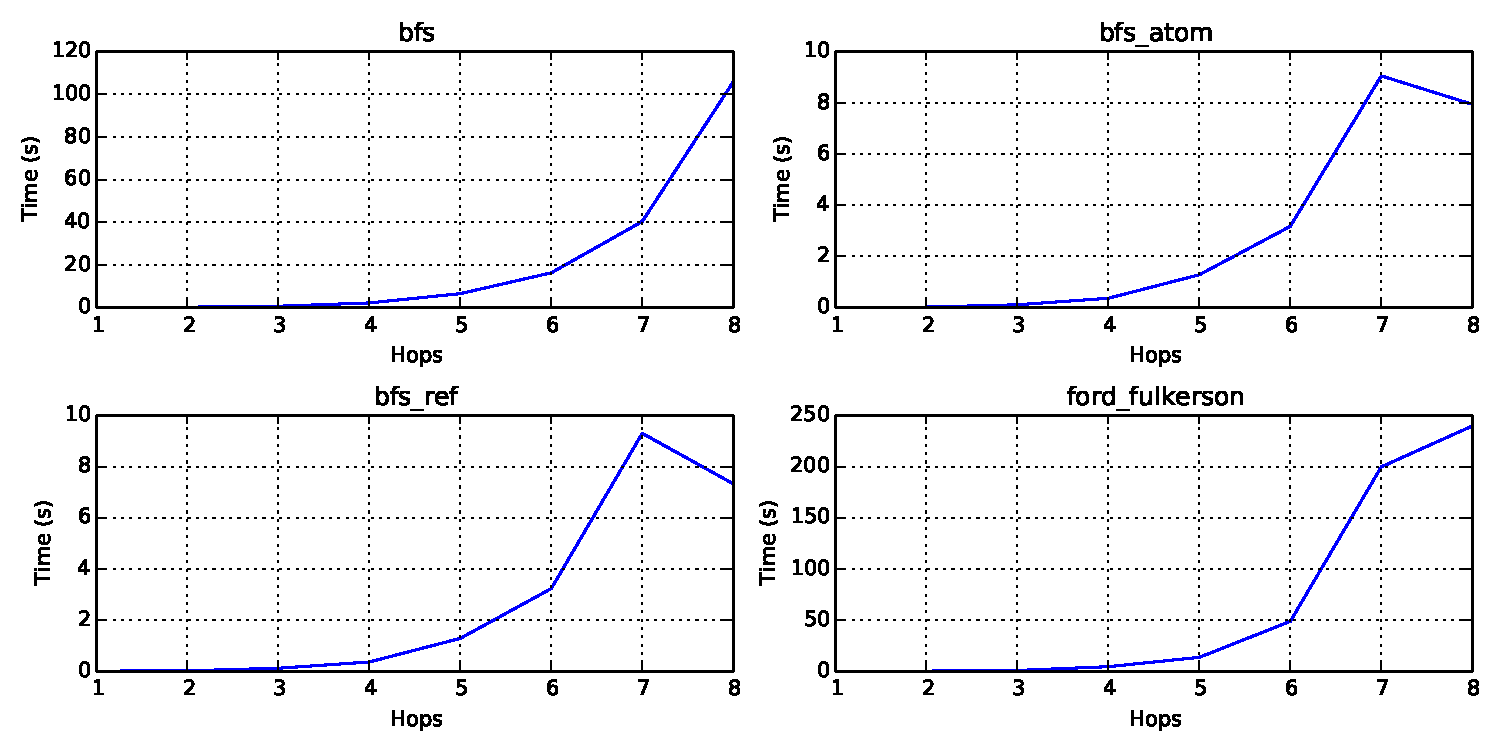
\includegraphics[scale=0.5]{images/methods-subplots}
					
					\caption{Growth of graph search times based on number of hops, plotted separately}
					\label{fig:methods-subplots}
				\end{figure}
				
				\begin{figure}[!ht]
					\centering
					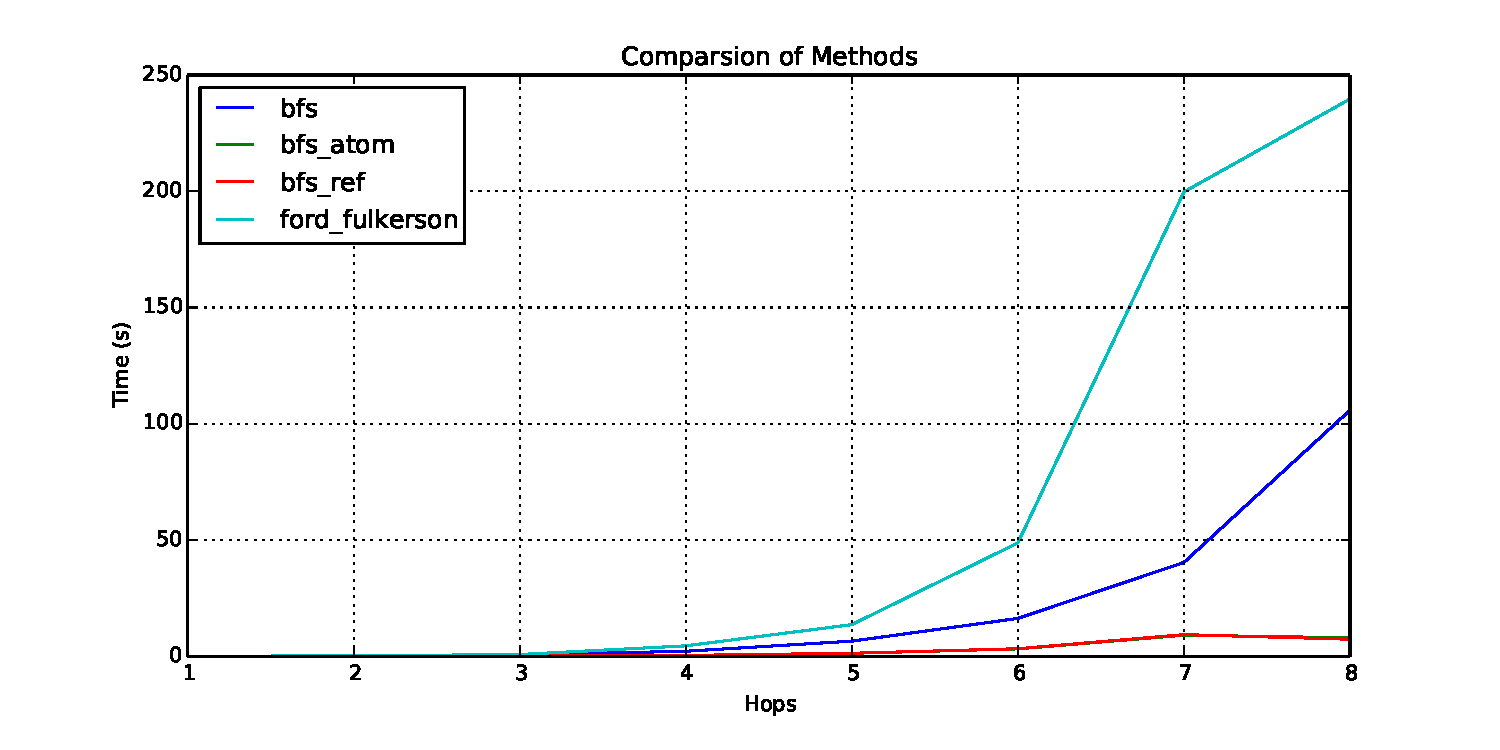
\includegraphics[scale=0.5]{images/methods-compared}
					
					\caption{Growth of graph search times based on number of hops, combined plot}
					\label{fig:methods-compared}
				\end{figure}
		
		\begin{itemize}
			\item Index speed
			\item Keyword search speed
			\item Graph search speed:
				\begin{itemize}
					\item Ford Fulkerson
					\item BFS
					\item Concurrent BFS using refs
					\item Concurrent BFS using atoms
				\end{itemize}
		\end{itemize}
	
	\section{Lessons learned}
		\begin{itemize}
			\item Simple algorithms are easier to parallelize
			\item STM is effective: transactions do not rollback (that much), so we observe impressive speed-up in concurrent versions.
			\item Fine tuning is beneficial: atom is better than ref.
			\item The clojure way: correctness first, runtime optimization latter (ref to atom is natural).
		\end{itemize}